\documentclass[11pt]{beamer}
\usetheme{Madrid}
\usecolortheme{default}
\usepackage{booktabs}
\usepackage{graphicx}
\usepackage{tikz}
\usetikzlibrary{shapes,arrows.meta,positioning,fit,backgrounds}

\title[Landslide Identification]{Landslide Identification Using Machine Learning}
\subtitle{M.Tech Project Presentation}
\author{Abhijit} % Placeholder for actual author name
\date{\today}

\begin{document}

% ---------------------------------------------------
% Slide 1: Title Slide
% ---------------------------------------------------
\begin{frame}
    \titlepage
    \begin{center}
        \textbf{Approach:} Two-Phase Pipeline — Deep Learning (CNN) + Probabilistic Model (HMM) \\
        \textbf{Tools Used:} Python, PyTorch, hmmlearn, OpenCV, Albumentations \\
        \textbf{Hardware:} NVIDIA RTX 2000 Ada Generation GPU, CUDA 12.4
    \end{center}
\end{frame}

% ---------------------------------------------------
% Slide 2: Problem Statement
% ---------------------------------------------------
\begin{frame}{Problem Statement}
    \textbf{What is the problem?}
    \begin{itemize}
        \item Landslides kill thousands of people every year and destroy infrastructure.
        \item Countries like India, Nepal, and China are highly affected.
        \item Manual satellite image analysis is slow, expensive, and scales poorly.
    \end{itemize}
    \vspace{0.3cm}
    \textbf{What we want to solve:}
    \begin{itemize}
        \item Automatically detect landslides in satellite images.
        \item Identify the specific \textit{type} of landslide.
        \item Predict future occurrences based on regional history.
    \end{itemize}
    \vspace{0.3cm}
    \textbf{Why this is important:} Early detection saves lives; combining visual detection with temporal prediction provides a comprehensive risk profile.
\end{frame}

% ---------------------------------------------------
% Slide 3: How This Project is Different
% ---------------------------------------------------
\begin{frame}{How This Project is Different}
    \begin{table}[]
        \centering
        \resizebox{\textwidth}{!}{
        \begin{tabular}{@{}ll@{}}
            \toprule
            \textbf{Existing Systems} & \textbf{Our System} \\ \midrule
            Use only NDVI or change detection & Classifies landslide type and predicts future events \\
            Manual feature engineering (SVM/RF) & Uses deep CNN that learns features directly \\
            Segmentation only (U-Net) & Combines image classification (Phase 1) with HMM (Phase 2) \\
            Binary output (Yes/No) & Full risk report: type, probability, peak risk month, forecast \\ \bottomrule
        \end{tabular}
        }
    \end{table}
    \vspace{0.3cm}
    \textbf{Key Difference:} Two independent phases working together — Phase 1 handles visual identification, Phase 2 handles temporal risk forecasting based on 28 years of data.
\end{frame}

% ---------------------------------------------------
% Slide 4: Dataset Collection
% ---------------------------------------------------
\begin{frame}{Dataset Collection}
    \textbf{Phase 1 Dataset — HR-GLDD (Image Classification)}
    \begin{itemize}
        \item \textbf{Source:} Zenodo (DOI: 7189381) - High-res satellite patches.
        \item \textbf{Preprocessing:} Converted NumPy arrays to multi-class JPEG directories (Non-Landslide, Rockfall, Mudflow, Debris Flow, Rotational Slide, Translational Slide).
        \item \textbf{Total Images:} \textasciitilde 3,439 images across Train/Val/Test splits.
    \end{itemize}
    \vspace{0.3cm}
    \textbf{Phase 2 Dataset — NASA Global Landslide Catalog (HMM)}
    \begin{itemize}
        \item \textbf{Source:} NASA Open Data Portal
        \item \textbf{Records:} 9,471 real landslide events (1988–2016) across 141 countries.
        \item \textbf{Features:} Event date, country, landslide type, trigger, size.
    \end{itemize}
\end{frame}

% ---------------------------------------------------
% Slide 5: System Architecture (Overview)
% ---------------------------------------------------
\begin{frame}{System Architecture (Overview)}
\begin{center}
    \resizebox{\textwidth}{!}{
    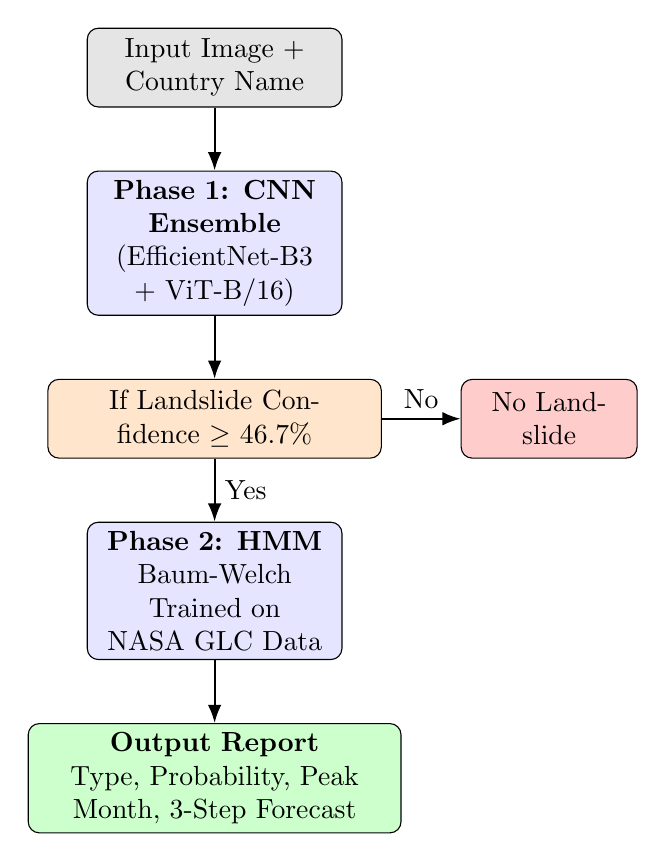
\begin{tikzpicture}[
        node distance=0.8cm and 1cm,
        box/.style={draw, rectangle, rounded corners, align=center, fill=blue!10, text width=3cm, minimum height=1cm},
        arrow/.style={-Latex, thick}
    ]
        % Inputs
        \node[box, fill=gray!20] (input) {Input Image + Country Name};
        
        % Phase 1
        \node[box, below=of input] (phase1) {\textbf{Phase 1: CNN Ensemble}\\(EfficientNet-B3 + ViT-B/16)};
        \node[box, below=of phase1, fill=orange!20, text width=4cm] (decision) {If Landslide Confidence $\ge$ 46.7\%};
        
        % Phase 2
        \node[box, below=of decision] (phase2) {\textbf{Phase 2: HMM}\\Baum-Welch Trained on NASA GLC Data};
        
        % Outputs
        \node[box, below=of phase2, fill=green!20, text width=4.5cm] (output) {\textbf{Output Report}\\Type, Probability, Peak Month, 3-Step Forecast};
        
        % Connections
        \draw[arrow] (input) -- (phase1);
        \draw[arrow] (phase1) -- (decision);
        \draw[arrow] (decision) -- node[right] {Yes} (phase2);
        \draw[arrow] (phase2) -- (output);
        
        % No branch
        \node[box, right=of decision, fill=red!20, text width=2cm] (no_ls) {No Landslide};
        \draw[arrow] (decision) -- node[above] {No} (no_ls);
        
    \end{tikzpicture}
    }
\end{center}
\end{frame}

% ---------------------------------------------------
% Slide 6: Phase 1 — CNN Architecture
% ---------------------------------------------------
\begin{frame}{Phase 1 — CNN Architecture (Detail)}
    \textbf{Primary Model: EfficientNet-B3}
    \begin{itemize}
        \item Pretrained on ImageNet (1.2M images).
        \item Replaced classification head for multi-class output.
    \end{itemize}
    \textbf{Secondary Model: ViT-B/16 (Vision Transformer)}
    \begin{itemize}
        \item Leverages attention mechanisms for global image context.
    \end{itemize}
    \textbf{Training Strategy \& Fusion}
    \begin{itemize}
        \item Transfer learning: Warm-up frozen layers, then differential learning rates.
        \item Data Augmentation: Grid distortion, coarse dropout, color jitter.
        \item Ensemble Fusion: Weighted probability sum (e.g., 60\% EffNet + 40\% ViT). Includes Temperature Scaling ($T \approx 1.15$) for calibration.
    \end{itemize}
\end{frame}

% ---------------------------------------------------
% Slide 7: Phase 2 — HMM Architecture
% ---------------------------------------------------
\begin{frame}{Phase 2 — HMM Architecture (Detail)}
    \textbf{Hidden Markov Model (CategoricalHMM)}
    \begin{itemize}
        \item Models sequential data, assuming hidden geological "regimes" produce visible landslide events.
        \item \textbf{Setup:} 8 hidden states, 42 combined observations (7 types $\times$ 6 triggers).
        \item \textbf{Training:} Baum-Welch (EM) algorithm over 112 country-level sequences.
    \end{itemize}
    \vspace{0.3cm}
    \textbf{How Prediction Works:}
    \begin{enumerate}
        \item \textbf{Current Type:} Viterbi decoding finds the likely regime.
        \item \textbf{Probability:} Derived from sequence log-likelihood.
        \item \textbf{Future Forecast:} Transition matrix multiplied $N$ times.
    \end{enumerate}
\end{frame}

% ---------------------------------------------------
% Slide 8: Results — Progression
% ---------------------------------------------------
\begin{frame}{Phase 1 Results \& Progression}
    \begin{table}[]
        \centering
        \resizebox{\textwidth}{!}{
        \begin{tabular}{@{}lcccc@{}}
            \toprule
            \textbf{Metric} & \textbf{AlexNet (Scratch)} & \textbf{AlexNet (Pretrained)} & \textbf{EfficientNet-B3} & \textbf{Ensemble (Final)} \\ \midrule
            Accuracy & 78.54\% & 80.11\% & 79.97\% & \textbf{82.40\%} \\
            Precision & 62.06\% & 66.67\% & 63.71\% & \textbf{68.03\%} \\
            Recall & 74.41\% & 68.25\% & 78.20\% & \textbf{78.67\%} \\
            F1-Score & 67.67\% & 67.45\% & 70.21\% & \textbf{72.97\%} \\
            ROC-AUC & 85.53\% & 88.33\% & 88.93\% & \textbf{89.83\%} \\ \bottomrule
        \end{tabular}
        }
    \end{table}
    \vspace{0.3cm}
    \textit{Note: The final ensemble utilizes an optimized decision threshold of 0.467.}
\end{frame}

% ---------------------------------------------------
% Slide 9: Conclusion & Future Work
% ---------------------------------------------------
\begin{frame}{Conclusion \& Future Improvements}
    \textbf{Achievements}
    \begin{itemize}
        \item Comprehensive pipeline analyzing both visual anomalies and historical sequential risks.
        \item High Phase 1 metrics (82.4\% Acc, 89.8\% AUC) paired with robust Phase 2 probabilistic forecasting.
    \end{itemize}
    \vspace{0.3cm}
    \textbf{Future Work}
    \begin{itemize}
        \item Integrate U-Net Segmentation for precise pixel-level localization.
        \item Incorporate NIR/Multispectral bands for vegetation damage detection.
        \item Expand dataset via Google Earth Engine and deploy as a real-time web monitoring tool.
    \end{itemize}
\end{frame}

\end{document}
